\chapter{Цель работы}

Цель работы - ознакомление с методами определения основных параметров и характеристик оптического волокна при его производстве.

\section{Краткие теоретические сведения}

Определение коэффициента затухания $\alpha$ в оптическом волокне (ОВ) 
производится с помощью анализатора оптического волокна ANDO и
 заключается в измерении интенсивности излучения $P_1$ заданной
  длины волны $\lambda$=1,3; 1,55 мкм, прошедшего через измеряемый образец 
  световода длиной $L$ и интенсивности излучения - $P_0$,
   прошедшего через отрезок световода известной длины (2м) с последующим расчетом по формуле:

\[
\alpha =\frac{10}{L} \cdot \lg{\frac{P_0}{P_1}}
\]



\begin{figure}[h!]
	\centering
	\caption{Схема анализатора ANDO}
	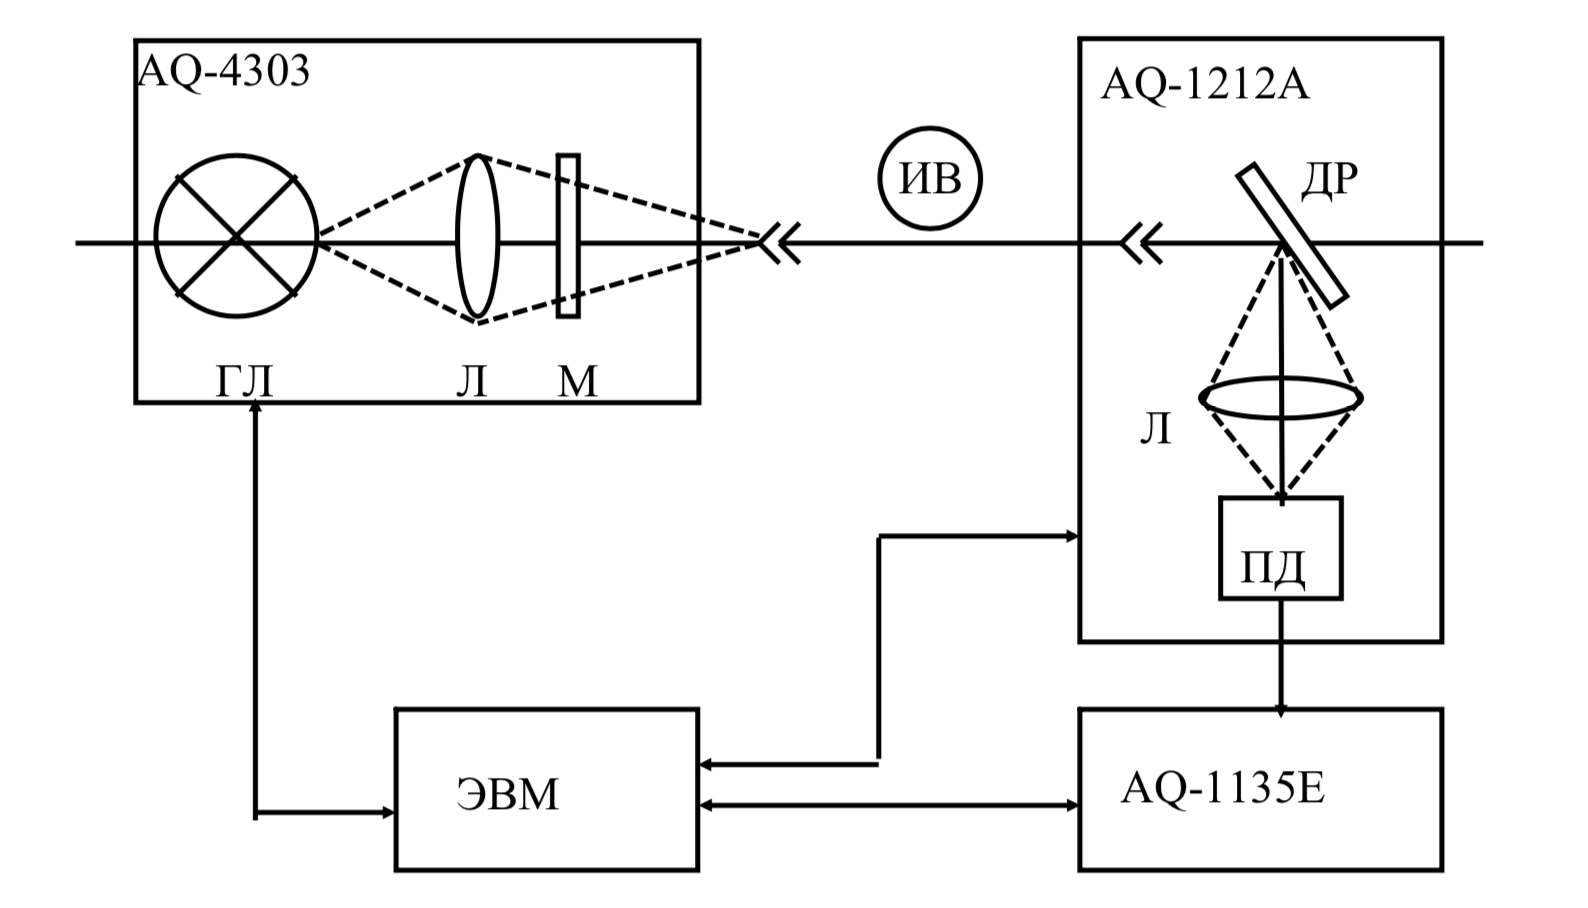
\includegraphics[width=.8\textwidth]{images/ando.png}
\end{figure}

AQ-4303 - источник излучения, ГЛ - галогеновая лампа, Л-линза, М - модулятор; 
ИВ - измеряемое волокно;
AQ-1212B - программируемый монохроматор, ДР - дифракционная решетка, Л - линза, ПД - приемник-демодулятор;
AQ-1135E - измеритель оптической мощности.

\chapter{Ход работы}

    \begin{table}[ht]
    	\caption{Условия}
	\begin{tabular}{|l|l|}
		\hline
		Номер варианта & 11		\\ \hline
		Длина образца, м & 2500 \\ \hline
		$P_o$, Вт & 20 \\ \hline
		Р, Вт (при $\lambda$=1,3мкм) & 19,99991 \\ \hline
		Р, Вт (при $\lambda$=1,55мкм) & 19,99995 \\ \hline
	\end{tabular}
\end{table}


\begin{figure}[h!]
	\centering
	\caption{Задание}
	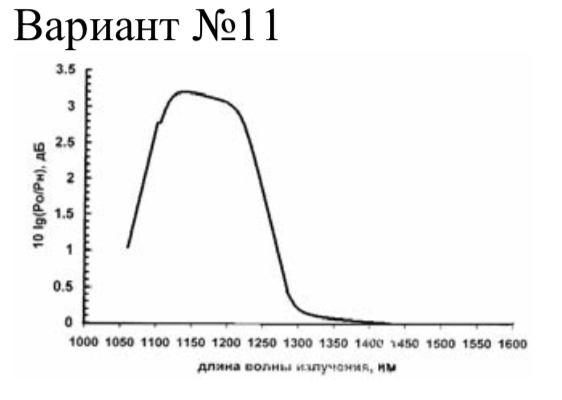
\includegraphics[width=.8\textwidth]{images/task.png}
\end{figure}

Графически определим длину волны отсечки:

\[
\lambda_\text{ДВО} = 1300 \text{ нм}
\]

Рассчитаем коэффициент затухания $\alpha$.

Для $\alpha$=1.3 мкм:

\[
\alpha_1 = \frac{10}{2500} \cdot \lg \frac{20}{19.9991} \approx 0.000000007817318
\]

Для $\alpha$=1.55 мкм:

\[
\alpha_2 = \frac{10}{2500} \cdot \lg \frac{20}{19.9995} \approx 0,00000000434295
\]

\begin{figure}[H]
	\centering
	\begin{tikzpicture}
	\begin{axis}[
	title={Зависимость $\alpha$ от температуры при длине волны 1,3 мкм},
	xlabel={$\alpha$, дБ/км},
	ylabel={$t$, $^\circ C$ },
	xmin=0.1, xmax=0.4,
	ymin=-60, ymax=110,
	legend pos=north west,
	ymajorgrids=true,
	grid style=dashed,
	]
	
	\addplot[
	color=blue,
	mark=square,
	smooth
	]
	coordinates {
(0.18, -50) (0.19, -40) (0.20, -30) (0.21, -20) (0.22, -10) (0.23, 0) (0.24, 10) (0.25, 20) (0.26, 30) (0.27, 40) (0.28, 50) (0.29, 60) (0.3, 70) (0.31, 80) (0.32, 90) (0.33, 100) 
	};
	
	
	\end{axis}
	\end{tikzpicture}
\end{figure}

\chapter{Выводы}

В результате работы была исследованы методы определения основных параметров и характеристик оптического волокна при его производстве. Результат расчётов совпадает с теоретическими сведениями. 